\chapter{Alternating-current circuits}

\section{A resonant circuit}

A circuit containing inductance, capacitance, and resistance was
one of the examples of the damped harmonic oscillator discussed in
Vol. 1, Chap. 7. Now we can see exactly what goes on in that system.
The circuit diagram in Fig. 8.1 represents such a ``series $RLC$'' circuit.

Let $Q$ be the charge, at time $t$, on the capacitor in this circuit. The
potential difference, or voltage across the capacitor, is $V$, which
obviously is the same as the voltage across the series combination
of inductor $L$ and resistor $R$. We take $V$ to be positive when the upper
capacitor plate is positively charged, and we define the positive current
direction by the arrow in Fig. 8.1. With the signs chosen that
way, the relations connecting charge $Q$, current $I$, and voltage across
the capacitor $V$ are:
\begin{equation}
  I=-\frac{\der Q}{\der t} \qquad
  Q = CV \qquad
  V=L\frac{\der I}{\der t}+RI
\end{equation}
We want to eliminate two of the three variables $Q$, $I$, and $V$. From
the first two equations we obtain $I = - C \der V/\der t$, and the third equation
becomes $V = -LC(\der^2V/\der t^2) - RC(\der V/\der t)$, or
\begin{equation}
  \frac{\der^2V}{\der t^2} + \left(\frac{R}{L}\right) \frac{\der V}{\der t} + \left(\frac{1}{LC}\right) V = 0
\end{equation}

This is a second-order differential equation with constant 
coefficients. We shall try a solution of the form
\begin{equation}
  V = A e^{-\alpha t}\cos\omega t
\end{equation}
where $A$, $\alpha$, and $\omega$ are constants. The first and second derivatives of
this function are:
\begin{align}
  \frac{\der V}{\der t} &=    A e^{-\alpha t}[-\alpha\cos\omega t-\omega\sin\omega t] \\
  \frac{\der^2V}{\der t^2} &= A e^{-\alpha t}[(\alpha^2-\omega^2)\cos\omega t+2\alpha\omega\sin\omega t]
\end{align}
% p. 275
Substituting back into Eq. 2, we cancel out the common factor $A e^{-\alpha t}$
and are left with
\begin{equation}
  (\alpha^2-\omega^2)\cos\omega t+2\alpha\omega\sin\omega t
       -\frac{R}{L}(\alpha\cos\omega t+\omega\sin\omega t)
       +\frac{1}{LC}\cos\omega t = 0
\end{equation}
This will be satisfied for all $t$ if, and only if, the coefficients of $\sin \omega t$
and $\cos\omega t$ are both zero. That is, we require:
\begin{equation}
  2\alpha\omega-\frac{R\omega}{L} = 0
\end{equation}
and
\begin{equation}
  \alpha^2-\omega^2-\alpha\frac{R}{L}+\frac{1}{LC} = 0
\end{equation}
The first of these equations gives a condition on $\alpha$:
\begin{equation}
  \alpha = \frac{R}{2L}
\end{equation}
while the second equation requires that:
\begin{equation}
  \omega^2 = \frac{1}{LC}-\alpha \frac{R}{L} + \alpha^2 = \frac{1}{LC}-\frac{R^2}{4L^2}
\end{equation}

Since our constant $\omega$ is a real number, $\omega^2$ cannot be negative.
Therefore we succeed in obtaining a solution of the form assumed in
Eq. 3 only if $R^2/4L^2\le 1/LC$. In fact it is the case of ``light
damping,'' that is, low resistance, that we want to examine, so we
shall assume that the values of $R$, $L$, and $C$ in the circuit are such that
the inequality $R < 2\sqrt{L/C}$ holds.

The function $A e^{-\alpha t}\cos\omega t$ is not the only possible solution.
$B e^{-\alpha t}\sin\omega t$ works just as well, with the same requirements, Eq. 9 and
Eq. 10, on $\alpha$ and $\omega$. The general solution is the sum of
these:
\begin{equation}
  V(t) = e^{-\alpha t}(A\cos\omega t+B\sin\omega t)
\end{equation}
V(t) = e'"'(A cos wt + B sin wt) (11)

The arbitrary constants $A$ and $B$ could be adjusted to fit initial
conditions. That is not very interesting. Whether the solution in
any given case involves the sine or the cosine function, or some 
superposition, is a trivial matter of how the clock is set. The essential
phenomenon is a damped sinusoidal oscillation.

% p. 276

The variation of voltage with time is shown in Fig. 8.2a. Of course,
this cannot really hold for all \emph{past} time. At some time in the past
the circuit must have been provided with energy somehow, and then
left running. For instance, the capacitor might have been charged,
with the circuit open, and then connected to the coil.

In Fig. 8.2b the time scale has been expanded and the dotted curve
showing the variation of the current $I$ has been added. For $V$ let us
take the damped cosine, Eq. 3. Then the current as a function of time
is given by:
\begin{equation}
  I = -C\frac{\der V}{\der t} = AC\omega\left(\sin\omega t+\frac{\alpha}{\omega}\cos\omega t\right)e^{-\alpha t}
\end{equation}
The ratio $\alpha/\omega$ is a measure of the damping. If $\alpha/\omega$ is very small,
many oscillations occur while the amplitude is decaying only a little.
For Fig. 8.2 we chose a case in which $\alpha/\omega\approx 0.04$. Then the cosine
term in Eq. 12 doesn't amount to much. All it does, in effect, is shift
the phase by a small angle, $\tan^{-1}(\alpha/\omega)$. So the current oscillation
is almost exactly one-quarter cycle out of phase with the voltage
oscillation.

The oscillation involves a transfer of energy back and forth from
the capacitor to the inductor, or from electric field to magnetic field.
At the times marked 1 in Fig. 8.2b all the energy is in the electric field.
A quarter-cycle later, at 2, the capacitor is discharged and nearly all
this energy is found in the magnetic field of the coil. Meanwhile, the
circuit resistance R is taking its toll, and as the oscillation goes on,
the energy remaining in the fields gradually diminishes.

The relative damping in an oscillator is often expressed by giving a
number called $Q$.\index{quality factor|see{Q}}\index{Q of an oscillator}
This was introduced in the general discussion of
harmonic oscillators in Vol. 1, Chap. 7. $Q$ (not to be confused with
the charge on the capacitor!) is said to stand for ``quality'' or ``quality
factor.'' In fact, no one calls it that; we just call it ``$Q$.'' The less
the damping, the larger the number $Q$. For an oscillator with frequency
$\omega$, $Q$ is the dimensionless ratio formed as follows:
\begin{equation}
  Q = \omega\frac{\text{energy stored}}{\text{average power dissipated}}
\end{equation}
Or you may prefer to remember that $Q$ is the number of radians of
the argument $\omega t$ (that is, $2\pi$ times the number of cycles) required for
the energy in the oscillator to diminish by the factor $1/e$.

% p. 278

In our circuit the stored energy is proportional to $V^2$ or $I^2$ and,
therefore, to $e^{-2\alpha t}$. The energy decays by $1/e$ in a time $t = 1/2\alpha$,
which covers $\omega/2\alpha$ radians. Hence for our $RLC$ circuit
\begin{equation}
  Q = \frac{\omega}{2\alpha} = \frac{\omega L}{R}
\end{equation}
As a rough estimate, what is the $Q$ of the oscillation represented in
Fig. 8.2?

Clearly, the general case we have just studied includes some simple
special cases. If $R = 0$ we have the completely undamped oscillator,
whose frequency $\omega_0$ is given by
\begin{equation}
  \omega_0 = \frac{1}{\sqrt{LC}}
\end{equation}
Mostly we deal with systems in which the damping is small enough
to be ignored in calculating the frequency. As Prob. 8.9 will 
demonstrate, damping has only a second-order effect on $\omega$.

For completeness we review brieffy what goes on in the 
overdamped circuit, in which $R > 2\sqrt{L/C}$. Equation 2 then has a solution
of the form $V = Ae^{-\beta t}$ for two values of $\beta$, the general solution
being
\begin{equation}
  V(t) = Ae^{-\beta_1 t}+Be^{-\beta_2 t}
\end{equation}
There are no oscillations, only a monotonic decay. In the special
case of ``critical'' damping, $R = 2\sqrt{L/C}$, $\beta_1=\beta_2$ and the solution
of the differential equation, Eq. 2, takes the form
\begin{equation}
  V(t) = (A + Bt)e^{-\beta t}
\end{equation}
This is the condition, for given L and C, in which the total energy
in the circuit is most rapidly dissipated. (See Prob. 8.8.)

You can see this whole range of behavior in Fig. 8.3, where $V(t)$ is
plotted for two underdamped circuits, a critically damped circuit,
and an overdamped circuit. The capacitor and inductor remain the
same; only the resistor is changed. The natural angular frequency
$\omega_0 = 1/\sqrt{LC}$ is $10^6\ \sunit^{-1}$ for this circuit, corresponding to a frequency
in cycles per second of $10^6/2\pi$, or 159 kHz.

The circuit is started off by charging the capacitor to a potential
difference of, say, 1 volt and then closing the switch at $t = 0$. That
is, $V = 1$ at $t = 0$ is one initial condition. Also, $I = 0$ at $t = 0$, because
the inductor will not allow the current to rise discontinuously.
Therefore, the other initial condition on $V$ is $\der V/\der t = 0$, at $t = 0$.
% p. 279
Notice that all four decay curves start the same way. In the heavily
damped case ($R = 600\ \text{ohms}$) most of the decay curve looks like
the simple exponential decay of an $RC$ circuit. Only the very beginning
where the curve is rounded over so that it starts with zero slope,
betrays the presence of the inductance $L$.

\section{Alternating current}

The resonant circuit we have just discussed contained no source
of energy and was, therefore, doomed to a \emph{transient}\index{transient behavior}
activity, an
oscillation that must sooner or later die out. In an 
alternating-current circuit we are concerned with a \intro{steady state}, a current and
voltage oscillating sinusoidally without change in amplitude. Some
oscillating electromotive force drives the system.

Let us apply an electromotive force $\emf = \emf_0 \cos \omega t$ to a circuit containing
inductance and resistance. We might generate $\emf$ by a
machine schematically like the one in Fig. 7.13, having provided
some engine or motor to turn the shaft at the constant angular
speed $\omega$. In Fig. 8.4 this electromotive force is represented as connected
into the circuit. We shall neglect any internal resistance in
the generator, or include it in $R$. We set the sum of potential drops
over the element of this circuit equal to the electromotive force $\emf$,
exactly as we did in developing Eq. 7.61. The equation governing
the current is then:
\begin{equation}
  L\frac{\der I}{\der t} + RI = \emf_0\cos\omega t
\end{equation}
Now there may be some transient behavior, depending on the
initial conditions, that is, on how and when the generator is switched
on. But we are interested only in the steady state, when the current
is oscillating obediently at the frequency of the driving force, with
the amplitude and phase necessary to keep Eq. 18 satisfied. To show
that this is possible, consider a current described by
\begin{equation}
  I = I_0 \cos (\omega t + \pot)
\end{equation}

To determine the constants $I_0$ and $\pot$, we put this into Eq. 18:
\begin{equation}
  -LI_0\omega \sin (\omega t + \pot) - RI_0 \cos (\omega t + \pot) = \emf_0 \cos \omega t
\end{equation}
The functions $\cos \omega t$ and $\sin \omega t$ can be separated out:
\begin{equation}
  -LI_0\omega(\sin\omega t\cos\pot + \cos\omega t\sin\pot)
     + RI_0(\cos\omega t\cos\pot - \sin\omega t\sin\pot) = \emf_0 \cos\omega t
\end{equation}
% p. 280
Setting the coefficients of $\cos \omega t$ and $\sin \omega t$ separately equal to zero,
\begin{equation}
  -LI_0\omega \cos\pot - RI_0\sin\pot = 0
\end{equation}
which gives
\begin{align}
  \tan\pot = -\frac{\omega L}{R}& \\
  -LI_0\omega \sin\pot - RI_0\cos\pot - \emf_0 = 0
\end{align}
which gives
\begin{align}
\begin{split}
  I_0 &= \frac{\emf_0}{R\cos\pot-\omega L\sin\pot} \\
      &= \frac{\emf_0}{R(\cos\pot+\sin\pot\tan\pot)} = \frac{\emf_0\cos\pot}{R}
\end{split}  
\end{align}
or since
\begin{align}
  \cos\pot &= \frac{R}{\sqrt{R^2+\omega^2L^2}}   \qquad (\text{from Eq. 23}) \\
  I_0 &= \frac{\emf_0}{\sqrt{R^2+\omega^2L^2}}
\end{align}

In Fig. 8.5 the oscillations of $\emf$ and $I$ are plotted on the same graph.
Since $\pot$ is a negative angle, the current reaches its maximum a bit
\emph{later} than the electromotive force. One says, ``The current lags the
voltage in an inductive circuit.'' The quantity $\omega L$ which has the
dimensions of resistance and can be expressed in ohms is called the
\intro{inductive reactance}.\index{reactance!inductive}

If we replace the inductor $L$ by a capacitor $C$, as in Fig. 8.6, we
have a circuit governed by the equation
\begin{equation}
  -\frac{Q}{C} + RI = \emf_0\cos\omega t
\end{equation}
We consider the steady-state solution
\begin{equation}
  I = I_0 \cos (\omega t + \pot)
\end{equation}
Since $I=-\der Q/\der t$, we have
\begin{equation}
  Q = -\int I\:\der t = -\frac{I_0}{\omega}\sin(\omega t+\pot)
\end{equation}
Note that in going from $I$ to $Q$ by integration, there is no question
of adding a constant of integration, for we know that $Q$ must oscillate
symmetrically about zero in the steady state.

% p. 281

Substituting back into Eq. 28 leads to
\begin{equation}
  \frac{I_0}{\omega C} \sin(\omega t+\pot) + R I_0\cos(\omega t+\pot) = \emf_0\cos\omega t
\end{equation}
Just as before, we obtain conditions on $\pot$ and $I_0$ by requiring that the
coefficients of $\cos \omega t$ and $\sin \omega t$ separately vanish. In this case, the
results are:
\begin{equation}
  \tan\pot = \frac{1}{R\omega C}  
\end{equation}
and
\begin{equation}
  I_0 = \frac{\emf_0}{R^2+(1/\omega C)^2}
\end{equation}
Notice that the phase angle is now positive. As the saying goes, the
current ``leads the voltage'' in a capacitive circuit. What this means
is apparent in the graph of Fig. 8.7.

Mathematically speaking, the function
\begin{equation}
  I = \frac{\emf_0}{\sqrt{R^2+\omega^2L^2}}\cos\left(\omega t-\tan^{-1}\frac{\omega L}{R}\right)
\end{equation}
is a \intro{particular integral} of the differential equation, Eq. 18. To this
could be added a \intro{complementary function}, that is, any solution of
the homogeneous differential equation
\begin{equation}
  L\frac{\der I}{\der t} + RI = 0
\end{equation}
Now this is just Eq. 7.65, whose solution we found, in Sec. 7.9, to be
an exponentially decaying function,
\begin{equation}
  I \sim e^{-(R/L)t}
\end{equation}
The physical significance is this: A transient, determined by some
initial conditions, is represented by a decaying component of $I (t)$,
of the form of Eq. 36. After a time $t \gg L/R$, this will have vanished
leaving only the steady sinusoidal oscillation at the driving frequency,
represented by the particular integral, Eq. 34.

The similarity of our results for the $RL$ circuit and the $RC$ circuit
suggests a way to look at the inductor and capacitor in series.
Suppose an alternating current $I = I_0 \cos (\omega t + \pot)$ is somehow
% p. 282
caused to flow through such a combination (shown in Fig. 8.8). The
voltage across the inductor, $V_L$, will be:
\begin{equation}
  V_L = L\frac{\der I}{\der t} = -I_0\omega L\sin(\omega t+\pot)
\end{equation}
The Voltage $V_C$ across the capacitor, with sign consistent with the sign
of $V_L$, is
\begin{equation}
  V_C = -\frac{Q}{C} = -\frac{1}{C}\int I\:\der t = \frac{I_0}{\omega C}\sin(\omega t+\pot)
\end{equation}
The voltage across the combination is then
\begin{equation}
  V = V_L+V_C = -\left(\omega L-\frac{1}{\omega C}\right)I_0\sin(\omega t+\pot)
\end{equation}
\emph{For a given $\omega$}, the combination is evidently equivalent to a single 
element, either an inductor or a capacitor, depending on whether the
quantity $\left(\omega L-\frac{1}{\omega C}\right)$ is positive or negative. Suppose, for example,
that $\omega L>\frac{1}{\omega C}$.  Then the combination is equivalent to an inductor
$L'$ such that
\begin{equation}
  \omega L' = \omega L-\frac{1}{\omega C}
\end{equation}
\emph{Equivalence} means \emph{only} that the relation between current and
voltage, for steady oscillation at the particular frequency $\omega$, is the
same. This allows us to replace $L$ and $C$ by $L'$ in any circuit driven
at this frequency.

This can be applied to the simple $RLC$ circuit in Fig. 8.9. We need
only recall Eqs. 23 and 27, the solution for the $RL$ circuit driven by
the electromotive force $\emf_0 \cos \omega t$, and replace $\omega L$ by $\omega L - 1/\omega C$:
\begin{align}
  I &= \frac{\emf_0}{\sqrt{R^2+(\omega L - 1/\omega C)^2}}\cos(\omega t+\pot) \\
  \tan\pot &= \frac{1}{R\omega C}-\frac{\omega L}{R}
\end{align}
For fixed amplitude $\emf_0$ of the electromotive force, and given circuit
elements $L$, $C$, and $R$, we get the greatest current when the driving
frequency $\omega$ is such that
\begin{equation}
  \omega L - \frac{1}{\omega C} = 0
\end{equation}
% p. 283
which is the same as saying that $\omega = 1/\sqrt{LC}=\omega_0$, the resonant
frequency of the undamped $LC$ circuit. In that case Eq. 39 reduces to
\begin{equation}
  I =  \frac{\emf_0\cos\omega t}{R}
\end{equation}
This is exactly the current that would flow if the circuit contained
the resistor alone.

As an example, consider the circuit of Fig. 8.3a, connected now
to a source or generator of alternating emf, $\emf = \emf_0 \cos \omega t$. The driving
frequency $\omega$ may be different from the resonant frequency
$\omega_0 = 1/\sqrt{LC}$, which, for the given capacitance (0.01 microfarads)
and the inductance (100 microhenrys), is $10^6\ \text{radians}/\sunit$
(or $10^6/2\pi\ \text{cycles}/\sunit$).
Figure 8.10 shows the amplitude of the oscillating 
current, as a function of the driving frequency $\omega$, for three different
% p. 284
values of the resistance $R$. It is assumed that the amplitude $\emf_0$
of the emf is 100 volts in each case. Notice the resonance peak at
$\omega = \omega_0$, which is most prominent and sharp for the lowest resistance
value. This is the same value of $R$ for which, running as a damped
oscillator without any driving emf, the circuit behaved as shown in
the top graph of Fig. 8.3b.

The $Q$ of the circuit, defined by Eq. 14
as $\omega_0L/R,$\footnote{The $\omega$ in Eq. 14 was the frequency of the
freely decaying damped oscillator, practically
the same as $\omega_0$ for moderate or light damping. We use $\omega_0$ here in the definition
of $Q$. In the present discussion $\omega$ is \emph{any} frequency we may choose to apply to this circuit.
}
is $\frac{(10^{6}\times10^{-4})}{20}$, or 5, in this case.
Generally speaking, the higher the $Q$ of a circuit,
the narrower and higher the peak of its response as a function of
driving frequency $\omega$. To be more precise, consider frequencies in
the neighborhood of $\omega_0$, writing $\omega = \omega_0 + \Delta\omega$. Then to first order
in $\Delta\omega/\omega_0$, the expression 
$\omega L - 1/\omega C$ which occurs in the 
denominator in Eq. 41 can be approximated this way:
\begin{equation}
  \omega L-\frac{1}{\omega C} = \omega_0 L \left(1+\frac{\Delta\omega}{\omega_0}\right)
          - \frac{1}{\omega_0 C(1+\Delta\omega/\omega_0)}
\end{equation}
and since $\omega_0$ is $1/\sqrt{LC}$, this becomes
\begin{equation}
  \omega_0 L \left[1+\frac{\Delta\omega}{\omega_0}-\frac{1}{1+\Delta\omega/\omega_0}\right]
    \approx \omega_0 L\left(2\frac{\Delta\omega}{\omega_0}\right)
\end{equation}
Exactly at resonance, the quantity inside the square root sign in
Eq. 41 is just $R^2$. As $\omega$ is shifted away from resonance the quantity
under the square root will have doubled when $|\omega L - 1/\omega C| = R$,
or when, approximately,
\begin{equation}
  \frac{2\Delta\omega}{\omega_0} = \frac{R}{\omega_0 L} = \frac{1}{Q}
\end{equation}
This means that the current amplitude will have fallen to $1/\sqrt{2}$ times
the peak when $\Delta\omega/\omega_0 = 1/2Q$. These are the ``half-power'' points,
because the energy, or power is proportional to the amplitude
squared, as we shall explain in Sec. 8.5. One often expresses the
width of a resonance peak by giving the full width between half-
power points. Evidently that is just $1/ Q$ times the resonant frequency
itself. Circuits with very much higher $Q$ than this one are
quite common. A radio receiver may select a particular station and
% p. 285
discriminate against others by the help of a resonant circuit with a $Q$
of several hundred. It is quite easy to make a microwave resonant
circuit with a $Q$ of $10^4$, or even $10^5$.

The angle $\pot$, which expresses the relative phase of the current and
emf oscillations, varies with frequency in the manner shown in
Fig. 8.11. At a very low frequency the capacitor is the dominant
hindrance to the flow of current, and $\pot$ is positive. At resonance, $\pot = 0$.
The higher the $Q$, the more abruptly $\pot$ shifts from positive to negative
angles as the frequency is raised through $\omega_0$.

\section{Alternating-current networks}

An alternating-current network is any collection of resistors,
capacitors, and inductors in which currents flow that are oscillating
steadily at the constant frequency to. One or more electromotive
forces, at this frequency, drive the oscillation. Figure 8.12 is a diagram
of one such network. The source of alternating electromotive
force is represented by the symbol 
\raisebox{-0.1\height}{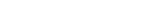
\includegraphics{ch08/figs/ac-emf-source}}.
In a branch of the network,
for instance the branch that includes the inductor $L_2$, the current as
a function of time is
\begin{equation}
  I_2 = I_{02} \cos (\omega t + \pot_2) 
\end{equation}
Since the frequency is a constant for the whole network, two 
numbers, such as the amplitude $I_{02}$ and the phase constant $\pot_2$ above, are
enough to determine for all time the current in a particular branch.
% p. 286
Similarly, the voltage across a branch oscillates with a certain
amplitude and phase:
\begin{equation}
  V_2 = V_{02} \cos (\omega t + \theta_2) 
\end{equation}

If we have determined the currents and voltages in all branches of
a network, we have analyzed it completely. To find them by constructing
and solving all the appropriate differential equations is
possible, of course; and if we were concerned with the transient behavior
of the network, we might have to do something like that. For
the steady state, however, we can use a far simpler and more elegant
method. It is based on two ideas:
\begin{enumerate}[(i)]
\item An alternating current or voltage can be represented by a
      complex number.
\item Any one branch or element of the circuit can be 
      characterized, at a given frequency, by the relation between the
      voltage and current in that branch.
\end{enumerate}

The first idea exploits that remarkable mathematical identity
\begin{equation}
  e^{i\theta} = \cos\theta+i\sin\theta
\end{equation}
with $i^2 = -1$. To carry it out we adopt the following \emph{rule} for the
representation:

\begin{framed}
An alternating current $I_0 \cos (\omega t + \pot)$ is to be \emph{represented
by} the complex number $I_0e^{i\pot}$, that is, the number whose real
part is $I_0 \cos \pot$ and whose imaginary part is $I_0 \sin \pot$.

Going the other way, if the complex number $x + iy$ \emph{represents}
a current $I$, then the current as a function of time is given
by the real part of the product $(x + iy)e^{i\omega t}$.
\end{framed}

Figure 8.13 is a reminder of this two-way correspondence. Since
a complex number $z = x + iy$ can be graphically represented on the
two-dimensional plane, it is easy to visualize the phase constant as
the angle $\tan^{-1} y/x$, and the amplitude $I_0$ as the modulus
$\sqrt{x^2+y^2}$.

What makes all this useful is the following fact: \emph{The representation
of the sum of two currents is the sum of their representations}. Consider
the sum of two currents $I_1$ and $I_2$ that meet at a junction of wires in
Fig. 8.12. At any instant of time $t$ the sum of the currents is:
\begin{align}
\begin{split}
  I_1+I_2 &= I_{01}\cos(\omega t+\pot_1) + I_{02}\cos(\omega t+\pot_2) \\
          &=  (I_{01}\cos\pot_1+I_{02}\cos\pot_2)\cos\omega t
             -(I_{01}\sin\pot_1+I_{02}\sin\pot_2)\sin\omega t
\end{split}
\end{align}
% p. 287
On the other hand, the sum of the complex numbers that, according
to our rule, represent $I_1$ and $I_2$ is:
\begin{equation}
  I_{01}e^{i\pot_1}+I_{02}e^{i\pot_2}
   =  (I_{01}\cos\pot_1+I_{02}\cos\pot_2)
    +i(I_{01}\sin\pot_1+I_{02}\sin\pot_2)
\end{equation}
If you multiply the right-hand side of Eq. 52 by $(\cos \omega t + i \sin \omega t)$
and take the real part of the result, you will get just what appears or
the right in Eq. 51.

This means that instead of adding or subtracting the periodic functions
of time themselves, we can add or subtract the complex numbers
that represent them. Or putting it another way, the algebra of alternating
currents turns out to be the same as the algebra of complex
numbers, in respect to addition. The correspondence does \emph{not} extend
to multiplication. The complex number $I_{01}I_{02}e^{i(\pot_1+\pot_2)}$ does \emph{not}
represent the product of the two current functions in Eq. 51.

However, it is only the addition of currents and voltages that we
need to carry out in analyzing the network. For example, at the
junction where $I_1$ meets $I_2$ in Fig. 8.12, there is the physical requirement
that \emph{at every instant} the net flow of current into the junction
shall be zero. Hence the condition
\begin{equation}
  I_1+I_2+I_3 = 0
\end{equation}
must hold, where $I_1$, $I_2$, and $I_3$ are the \emph{actual periodic functions of
time}. Thanks to our correspondence, this can be expressed in the
% p. 288
simple algebraic statement that the sum of three complex numbers
is zero. Voltages can be handled in the same way. Instantaneously,
the sum of the voltage drops around any loop in the network must
equal the electromotive force in the loop at that instant. This condition
relating periodic voltage functions can likewise be replaced by
a statement about the sum of some complex numbers, the representations
of the various oscillating functions, $V_1(t)$, $V_2(t)$, etc.

\section{Admittance and impedance}

The relation between current flow in a circuit element and the
voltage across the element can be expressed as a relation between the
complex numbers that represent the voltage and the current. Look
at the inductor-resistor combination in Fig. 8.4. The voltage oscillation
is represented by $\emf_0$ and the current by $I_0e^{i\phi}$, where 
$I_0 = \emf_0/\sqrt{R^2+\omega^2L^2}$ and $\tan \pot = -\omega L/R$. The phase difference $\pot$ and
the ratio of current amplitude to voltage amplitude are properties
of the circuit at this frequency. We define a complex number $Y$ as
follows:
\begin{equation}
  Y=\frac{e^{i\phi}}{\sqrt{R^2+\omega^2L^2}} \qquad \text{with} \qquad
          \pot = \tan^{-1}\left(-\frac{\omega L}{R}\right)
\end{equation}
Then the relation
\begin{equation}
  I = YV
\end{equation}
holds, where $V$ is the complex number that represents the voltage
across the series combination of $R$ and $L$, and $I$ is the complex number
that represents the current. $Y$ is called the \intro{admittance}. The
same relation can be expressed with the reciprocal of $Y$, denoted by
$Z$ and called the impedance:\index{impedance}
\begin{equation}
  V = \left(\frac{1}{Y}\right)I = ZI
\end{equation}

Here we do make use of the product of two complex numbers, but
only one of the numbers is the representation of an alternating current
or Voltage. The other is the impedance 
or admittance.\footnote{Our algebra
thus contains two categories of complex numbers, those that represent
impedances, for example, and those that represent currents. The product of two
``impedance numbers,'' like the product of two ``current numbers,'' doesn't represent
anything.}

% p. 289

The impedance is measured in ohms. Indeed, if the circuit element
consisted of the resistance $R$ alone, the impedance would
be real and equal simply to $R$, so that Eq. 56 would resemble Ohm's
law for a direct-current circuit: $V = RI$.

The admittance of a resistanceless inductor is the imaginary
quantity $Y = -i/\omega L$. This can be seen by letting $R$ go to zero in
Eq. 54. The factor $-i$ shows that the current oscillation lags the
voltage oscillation by $\pi/2$ in phase. On the complex number 
diagram, if the voltage is represented by $V$ (Fig. 8.14b), the current
might be represented by $I$, located as shown there. For the capacitor,
$Y = i\omega C$, as can be seen from the expression for the current in
Fig. 8.7. In this case $V$ and $I$ are related as indicated in Fig. 8.14c.
The inset in each of the figures shows how the relative sign of $V$ and $I$
is to be specified. Unless that is done consistently, ``leading'' and
``lagging'' are meaningless. Note that we always define the positive
current direction so that a positive voltage applied to a resistor causes
positive current (Fig. 8.14a).

The properties of the three basic circuit elements are summarized
below:

\vspace{5mm}
\begingroup
\renewcommand*{\arraystretch}{2}
\begin{tabular}{|c|c|c|}
\hline
\emph{Symbol} & \emph{Admittance, $Y$} & \emph{Impedance, $Z=\frac{1}{Y}$} \\
\hline
\raisebox{-.3\height}{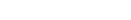
\includegraphics{ch08/figs/table-resistor}}
   & $\frac{1}{R}$
   & $R$ \\
\raisebox{-.3\height}{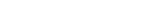
\includegraphics{ch08/figs/table-inductor}}
   & $\frac{-i}{\omega L}$
   & $i\omega L$ \\
\raisebox{-.3\height}{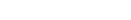
\includegraphics{ch08/figs/table-capacitor}}
   & $i\omega C$
   & $\frac{-i}{\omega C}$ \\
\hline
   & I=YV & V=ZI \\
\hline
\end{tabular}
\endgroup
\vspace{5mm}

We can build up any circuit from these elements. When elements
or combinations of elements are connected in parallel, it is convenient
to use the admittance, for in that case admittances add. In Fig. 8.15
two ``black boxes'' with admittances $Y_1$ and $Y_2$ are connected in
parallel. We have then
\begin{equation}
  I = I_1+I_2 = Y_1V+Y_2V = (Y_1+Y_2)V
\end{equation}
% p. 290
which implies that the equivalent single black box has an admittance
$Y = Y_1 + Y_2$. From Fig. 8.16 it will be obvious that the \emph{impedances}
add for elements connected in \emph{series}. It sounds as if we are talking
about a direct-current network! In fact, we have now reduced the
ac network problem to the dc network problem, with only this 
difference: the numbers we deal with are complex numbers.

As an example, let's look at the ``parallel $RLC$'' circuit in
Fig. 8.17. The combined admittance of the three parallel branches is
\begin{equation}
  Y = \frac{1}{R} + i\omega C - \frac{i}{\omega L}
\end{equation}
The voltage is simply $\emf_0$, so the complex current is
\begin{equation}
  I = YV = \emf_0\left[\frac{1}{R} \: + \: i\left(\omega C-\frac{1}{\omega L}\right)\right]
\end{equation}
The amplitude of the current oscillation is the modulus of the complex
number $I$, which is $\emf_0 [(1/R)^2 + (\omega C - 1/\omega L)^2]^{1/2}$, and the
phase angle is $\tan^{-1} (R\omega C - R/\omega L)$.

We can only deal in this way with \emph{linear} circuit elements, elements
in which the current is proportional to the voltage. In other words,
our circuit must be described by a linear differential equation. You
can't even define an impedance for a nonlinear element. Nonlinear
circuit elements are very important and interesting devices. You
have studied some in the laboratory, and you can see why they will
not readily yield to this kind of analysis.

This is all predicated, too, on the continuous oscillation at constant
frequency. The transient behavior of the circuit is a different
problem. However, for linear circuits the tools we have just developed
have some utility, even for transients. The reason is that by
superposing steady oscillations of many frequencies we can represent
a nonsteady behavior, and the response to each of the individual
frequencies can be calculated as if that frequency were present alone.
This can well be left for Volume III.

\section{Power and energy in alternating-current circuits}
If the voltage across a resistor $R$ is $V_0 \cos \omega t$, the current is
$I = (V_0/R) \cos \omega t$. The instantaneous power, that is the instantaneous
rate at which energy is being dissipated in the resistor is
\begin{equation}
  P = RI^2 = \frac{V_0^2}{R}\cos^2\omega t
\end{equation}
% p. 291
Since the average of $\cos^2\omega t$ over many cycles is $\frac{1}{2}$, the average power
dissipated in the circuit is
\begin{equation}
  \bar{P} = \frac{1}{2}\frac{V_0^2}{R}
\end{equation}
It is customary to express voltage and current in ac circuits by giving
not the amplitude but $1/\sqrt{2}$ times the amplitude. This is often called
the ``root-mean-square'' or, for short, ``rms'' value.\index{amplitude!rms}\index{rms}\index{root-mean-square}
That takes care
of the factor $\frac{1}{2}$ in Eq. 61, so that
\begin{equation}
  \bar{P} = \frac{V_\text{rms}^2}{R}
\end{equation}
For example, the common domestic line voltage in the United States, 120 volts, corresponds
to an \emph{amplitude} $120\sqrt{2}$ volts. The potential difference 
between the terminals of the electric outlet in your room (if the voltage
is up to normal) is
\begin{equation}
  V(t) = 170\cos 377t
\end{equation}
with $V$ in volts and $t$ in seconds. An ac ammeter is calibrated to read
$1\ \zu{A}$ when the current amplitude is 1.414 amperes.

In general, the instantaneous rate at which energy is delivered to
a circuit element is $VI$, the product of the instantaneous voltage and
current, with due regard to sign. Consider this aspect of the current
flow in the simple $LR$ circuit in Fig. 8.4. In Fig. 8.18 we have redrawn
the current and voltage graphs and added a curve proportional to
the product $VI$. Positive $VI$ means energy is being transferred into
the $LR$ combination from the source of electromotive force, or
generator. Notice that $VI$ is negative in certain parts of the cycle.
In those periods some energy is being returned to the generator.
This is explained by the oscillation in the energy stored in the magnetic
field of the inductor. This stored energy, $\frac{1}{2}LI^2$, goes through
a maximum twice in each full cycle.

The \emph{average} power, $\bar{P}$, corresponds to the horizontal dashed line.
To calculate its value, let's look at the product $VI$, with $V = \emf_0 \cos \omega t$
and $I = I_0\cos(\omega t+\pot)$:
\begin{align}
\begin{split}
  VI &= \emf_0I_0\cos\omega t \cos(\omega t+\pot) \\
     &= \emf_0I_0(\cos^2\omega t\cos\pot - \cos\omega t\sin\omega t\sin\pot)
\end{split}
\end{align}
% p. 292
The term proportional to $\cos\omega t\sin\omega t$ has a time average
zero, as is obvious if you write it as $\frac{1}{2}\sin2\omega t$, while
the average of $\cos^2\omega t$ is $\frac{1}{2}$.
Thus for the time average we have
\begin{equation}
  \bar{P} = \overline{VI} = \frac{1}{2}\emf_0I_0\cos\pot
\end{equation}
If both current and voltage are expressed as rms values, in volts and
amperes respectively,
\begin{equation}
  \underbrace{\bar{P}}_\text{(watts)}
        = \underbrace{V_\text{rms}}_\text{(volts)}
          \underbrace{I_\text{rms}}_\text{(amperes)}
          \cos\pot
\end{equation}
In this circuit all the energy dissipated goes into the resistance $R$.
Naturally, any real inductor has some resistance. For the purpose
of analyzing the circuit, we included that with the resistance $R$. Of
course the heat evolves at the actual site of the resistance.

To practice with the methods we developed in Sec. 8.4, we'll analyze
the circuit in Fig. 8.19a. A $10,000\ \text{ohm}$, $1\ \zu{W}$ resistor has been
connected up with two capacitors of capacitance 0.2 and 0.5 microfarads
($\mu\zu{F}$). We propose to plug this into the 120 V, 60 Hz outlet.
\emph{Question:} Will the 1 W resistor get too hot? In the course
of finding out whether the average power dissipated in $R$ exceeds the
1 W rating, we'll calculate some of the currents and voltages we
might expect to measure in this circuit. One way to work through the
circuit is outlined below.

\begin{enumerate}[(i)]

\item
  $\text{Admittance of $C_2$} = i\omega C_2 = (377)(2\times 10^{-7})i 
                               = 0.754\times 10^{-4}i\ \text{ohm}^{-1}$

\item $\text{Admittance of the resistor} = \frac{1}{R} = 10^{-4}\ \text{ohm}^{-1}$

\item Admittance of 
         \raisebox{-0.4\height}{\includegraphics{ch08/figs/rc-parallel}}
         $=\ 10^{-4}(1+0.754i)\ \text{ohm}^{-1}$

\item Impedance of 
         \raisebox{-0.4\height}{\includegraphics{ch08/figs/rc-parallel}}
         $=\frac{1}{10^{-4}(1+0.754i)}
          =\frac{10^4(1-0.754i)}{1^2+0.754^2}
          = (6360-4800i)\ \text{ohm}$

\item $\text{Impedance of $C_1$} = -\frac{i}{\omega C}
               = -\frac{i}{(377)(5\times 10^{-7})}
               = -5300i\ \text{ohm}$

\item $\text{Impedance of entire circuit} = (6360-10,100i)\ \text{ohm}$

\item $I_1 = \frac{120}{6360-10,100i} = \frac{120(6360+10,100i)}{(6360)^2+(10,100)^2}
           = (5.37+8.53i)\times 10^{-3}\ \zu{A}$

\end{enumerate}

\noindent Since we have used 120 volts, which is the rms voltage, we obtain the
rms current. That is, the modulus of the complex number $I_1$, which
is $[(5.37)^2+(8.53)^2]^{1/2}\times10^{-3}\ \zu{A}$ or 10.0 mA,
is the rms current. An ac milliammeter inserted in series
with the line would read 10 mA. This current has a phase angle
$\pot=\tan^{-1}(0.853/0.537)$ or 1.01 radians with respect to the line
voltage. The average power delivered to the entire circuit is then:

% FIXME -- had to do these Roman numerals by hand
\vspace{3mm}
\noindent (viii) $\bar{P}=(120\ \text{volts})(0.010\ \zu{A})\cos1.01=0.64\ \zu{W}$
\vspace{3mm}

\noindent In this circuit the resistor is the only dissipative element, so this must
be the average power dissipated in it. Just as a check, we can find
the voltage $V_2$ across the resistor:

\vspace{3mm}
\noindent (ix) $V_1=I_1\left(\frac{-i}{\omega C}\right) = (5.37+8.53i)(-5300i)10^{-3}
        =(45.2-28.4i)\ \zu{V}$
\vspace{3mm}

\noindent (x) $V_2=120-V_1=(74.8+28.4i)\ \zu{V}$
\vspace{3mm}

\noindent The current $I_2$ in $R$ will be in phase with $V_2$, of course, so the average
power in $R$ will be
\begin{equation}
  \bar{P} = \frac{V_2^2}{R} = \frac{(74.8)^2+(28.4)^2}{10^4} = 0.64\ \zu{W}
\end{equation}
which checks.

Thus the rating of the resistor isn't exceeded, for what that
assurance is worth. Actually, whether the resistor will get too hot
depends not only on the average power dissipated in it but also on how
easily it can get rid of the heat. The power rating of the resistor is
only a rough guide.
